\documentclass[10pt,twocolumn]{article}

\usepackage{iftex}
\ifXeTeX
  \usepackage{fontspec}
\else
  \usepackage[utf8]{inputenc}
  \usepackage[T1]{fontenc}
  \usepackage{lmodern}
\fi
\usepackage[letterpaper,margin=2cm,columnsep=0.8cm]{geometry}
\usepackage{graphicx}
\usepackage{booktabs}
\usepackage{amsmath}
\usepackage{titlesec}
\usepackage[colorlinks=true,linkcolor=blue,urlcolor=blue,citecolor=blue]{hyperref}

\graphicspath{{figures/}}

\titleformat{\section}{\large\bfseries}{\thesection.}{0.5em}{}
\titleformat{\subsection}{\normalsize\bfseries\itshape}{\thesubsection.-}{0.4em}{}
\titlespacing*{\subsection}{0pt}{2ex}{1.5ex}
\renewcommand{\refname}{Referencias}
\renewcommand{\figurename}{Figura}
\renewcommand{\tablename}{Tabla}
\setlength{\parskip}{0.4em plus 0pt minus 0pt}
\raggedbottom
\setlength{\parindent}{0pt}

\title{\textbf{LoL Champions Visual Data: Reconocer al Campeón\\a partir de su Splash Art}}
\author{Emilio López\\\small A01711977@tec.mx}
\date{}

\begin{document}

\twocolumn[
\begin{@twocolumnfalse}
\maketitle
\vspace{-1.5em}
\noindent\textbf{ABSTRACT} Este reporte muestra cómo construimos una red neuronal convolucional que reconoce a qué campeón de League of Legends pertenece una splash art, usando el dataset \textit{``League of Legends Champions Visual Data''}. El reto principal es que cada campeón tiene muy pocas imágenes, y entre sus skins cambian los colores, la ropa y el fondo, lo único que se mantiene es el propio campeón. Durante la limpieza encontramos y quitamos 174 splash arts grupales (la misma imagen etiquetada como campeones distintos) y 18 duplicados, y después de una primera iteración fallida con 107 campeones nos quedamos con los 38 que tienen al menos 15 imágenes limpias. Seguimos un proceso incremental de nueve versiones: una CNN desde cero (v1) se quedó en 0.105 de accuracy en validación, el aumento de datos con Dropout no la mejoró, y el transfer learning con EfficientNetB0, congelada y luego con fine-tuning, llegó a 0.200. El cambio que más ayudó fue dividir la splash en tres recortes de 384~px en lugar de aplastarla, lo que subió validación a 0.242 y el top-5 a 0.589. Después vimos que el color de las skins confunde al modelo, así que entrenamos y predecimos en escala de grises, lo que subió validación a 0.316. Como todas las versiones memorizaban train, suponíamos que el límite era la falta de datos, y para comprobarlo agregamos a train 380 fan arts y cosplays de los campeones. Con el mismo modelo, validación subió a 0.389 y el F1 macro de 0.278 a 0.374, lo que confirmó la hipótesis. Ese es nuestro modelo final, y llegó a 0.263 de accuracy, 0.516 de top-5 y 0.242 de F1 macro en test, contra 0.026 que daría el azar con 38 clases. Para la interfaz web reentrenamos esa misma configuración con todas las imágenes, pero ese modelo ya no se puede medir, así que las métricas que reportamos son las del modelo final.
\vspace{1.5em}
\end{@twocolumnfalse}
]

\section{Introducción}

League of Legends tiene más de 170 campeones, y cada uno tiene varias skins: versiones alternativas del personaje con otro diseño, otra ropa y otros colores. Cada skin viene con una splash art, una ilustración grande del campeón en una escena. Reconocer a un campeón en cualquiera de sus skins es fácil para alguien que juega, porque se fija en la silueta, el arma o las proporciones del personaje, pero para un modelo es bastante más difícil, ya que dos skins del mismo campeón pueden no compartir ni un solo color, y dos campeones distintos pueden tener skins de la misma temática y verse casi iguales.

El objetivo de este trabajo es construir, con TensorFlow y Keras, un clasificador de imágenes que reciba una splash art y diga a qué campeón pertenece, junto con su top 5 de campeones más probables. La idea no es solo llegar a un modelo que funcione, sino mostrar todo el proceso, desde cómo limpiamos los datos y por qué tomamos cada decisión, hasta lo que probamos que no funcionó y lo que nos enseñaron los errores del modelo sobre el problema.

Para eso seguimos un proceso incremental, empezamos con una CNN sencilla como aproximación inicial, y fuimos agregando una mejora a la vez (aumento de datos, transfer learning, fine-tuning, cambios en la entrada, fan arts y cosplays para tener más datos y reentrenamiento con todos los datos), midiendo el efecto de cada una en el conjunto de validación.

\section{Descripción del Dataset}

El dataset es \textit{League of Legends Champions Visual Data}, de Kaggle~\cite{dataset}. Tiene una carpeta por campeón (172 en total) con 5,872 archivos, de dos tipos:

\begin{itemize}
  \item \textbf{Íconos de habilidades} (archivos 00--04): 860 imágenes PNG de $64\times64$.
  \item \textbf{Splash arts} (archivos 05 en adelante): 2,076 imágenes JPG de $1215\times717$, una por skin. El archivo 05\_<CAMPEÓN> es siempre la skin original.
\end{itemize}

Además, cada imagen viene con una copia en escala de grises que termina en \_bw, así que el total de archivos es el doble.

El número de splash arts por campeón es muy desigual (Figura~\ref{fig:distribucion}). La media es de 12 por campeón, pero los campeones más recientes tienen solo 2 o 3 (Ambessa, Yunara, Hwei, Mel, Aurora) mientras que los más viejos llegan a 23. Esto ya nos adelantaba que la cantidad de datos iba a ser el problema principal.

\begin{figure}[h]
  \centering
  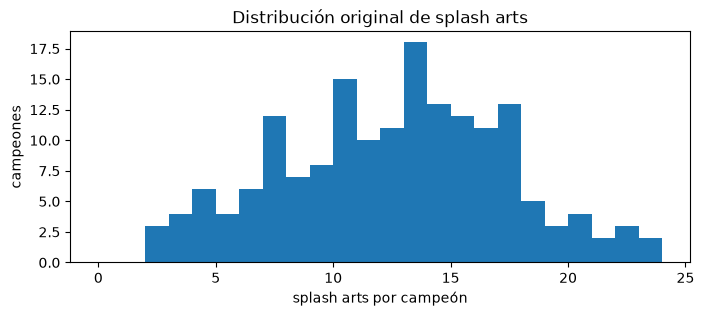
\includegraphics[width=\columnwidth]{distribucion_splash.png}
  \caption{Distribución original de splash arts por campeón.}
  \label{fig:distribucion}
\end{figure}

\section{Extracción y Limpieza de Datos}

\subsection{Íconos contra Splash Arts}

Lo primero que decidimos fue usar solo las splash arts. Los íconos de habilidades no muestran al campeón, son efectos, armas o símbolos de $64\times64$, así que en realidad son otro problema visual. Mezclarlos con las splash obligaría al modelo a aprender dos tareas distintas con muy pocos ejemplos de cada una.

\subsection{Splash Arts Grupales y Duplicados}

Al revisar las imágenes encontramos que algunas skins son grupales, o sea que la misma imagen muestra a varios campeones (por ejemplo, las skins de equipos de esports como DRX o SKT T1), y en el dataset esa imagen aparece copiada en la carpeta de cada uno (Figura~\ref{fig:grupales}). Para el modelo eso es la misma entrada con etiquetas distintas, algo imposible de aprender que además ensucia la evaluación.

También había imágenes repetidas dentro de un mismo campeón (por ejemplo, PRESTIGE\_KDA\_AHRI y PRESTIGE\_KDA\_AHRI\_2022). Si una cae en train y la otra en test, el resultado se infla, porque el modelo estaría ``reconociendo'' una imagen que ya vio.

Para detectar ambos casos usamos dos huellas por imagen:

\begin{itemize}
  \item \textbf{MD5}: detecta archivos idénticos byte por byte.
  \item \textbf{Average hash}: reduce la imagen a $16\times16$ en grises y marca qué pixeles están por encima de la media. Detecta imágenes casi iguales aunque tengan otra compresión o un recorte un poco distinto.
\end{itemize}

Si una huella se repetía entre campeones distintos la marcamos como grupal, y si se repetía dentro del mismo campeón, como duplicado. En total quitamos 174 splash grupales y 18 duplicados. Los campeones más afectados fueron Rakan y Xayah (7 grupales cada uno), que comparten casi todas sus skins.

\begin{figure}[h]
  \centering
  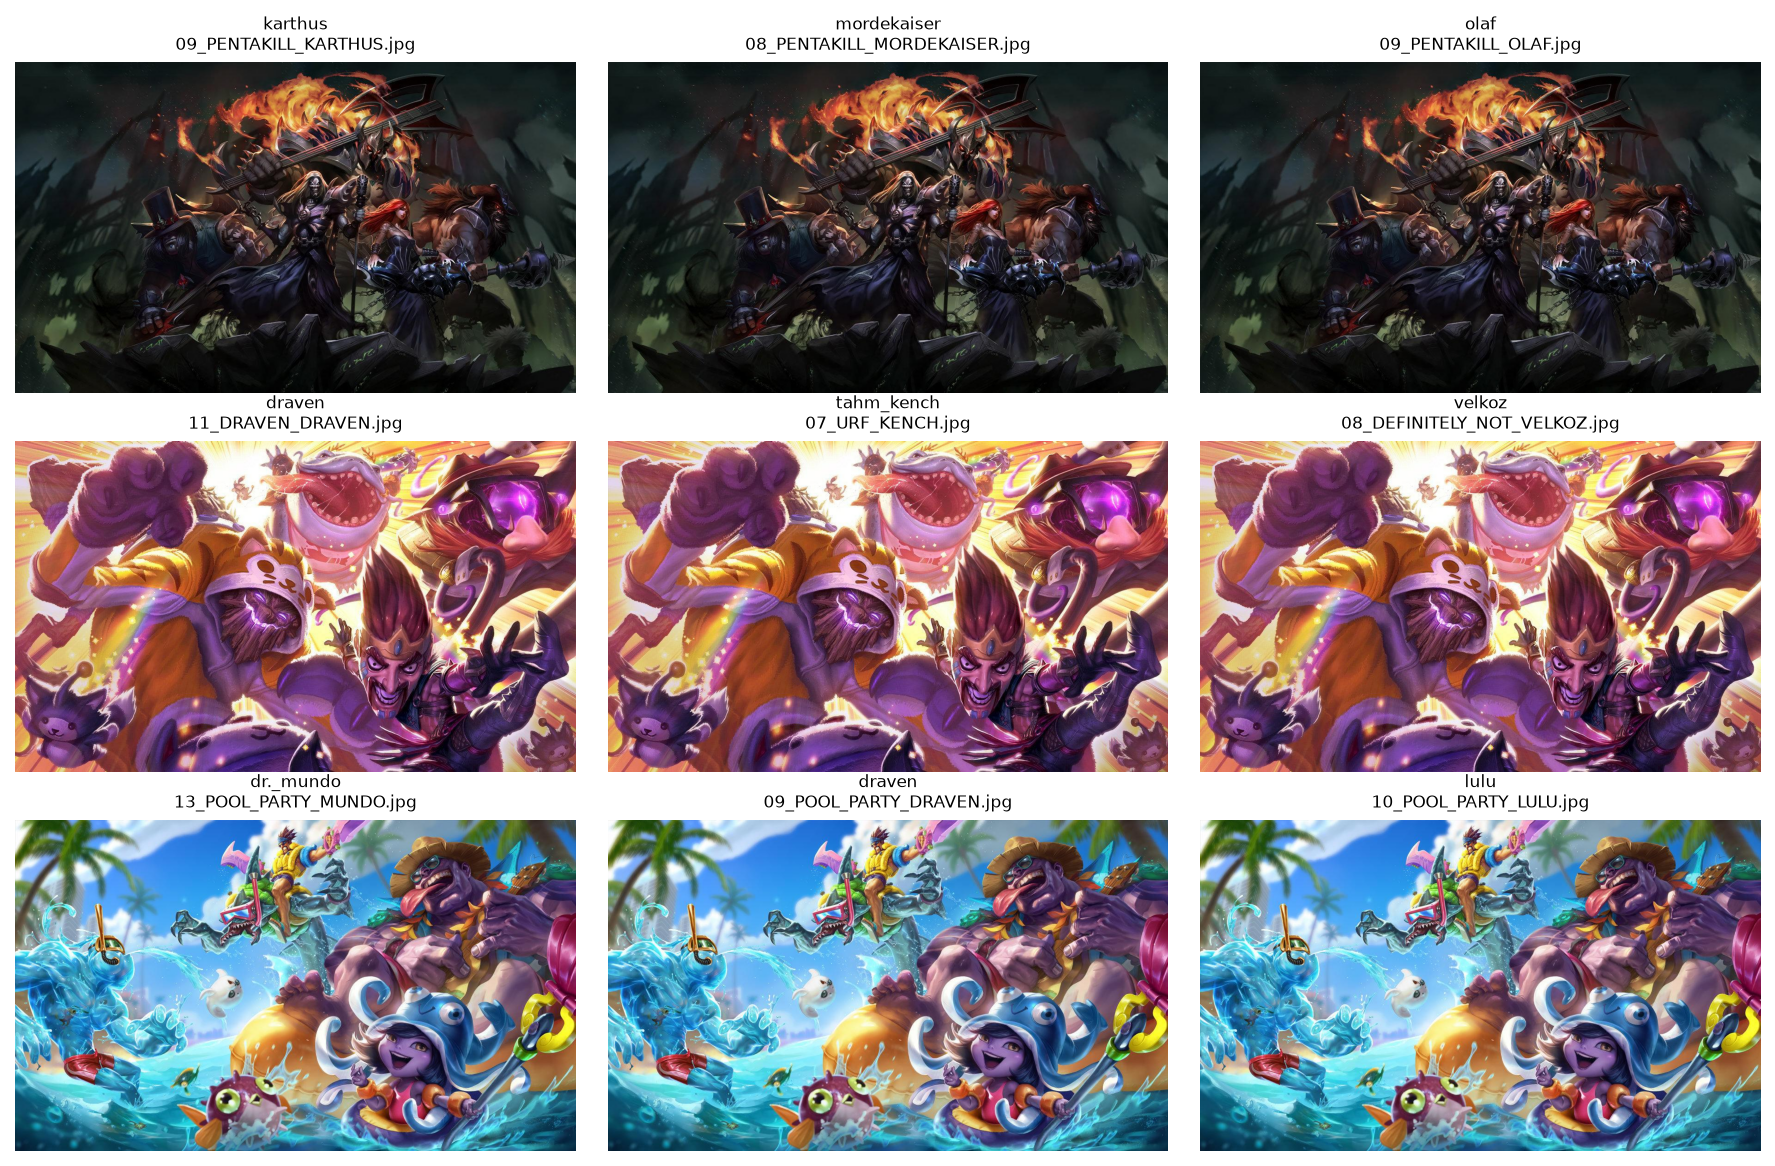
\includegraphics[width=\columnwidth]{splash_grupales.png}
  \caption{Ejemplos de splash arts grupales: la misma imagen aparece en la carpeta de cada campeón.}
  \label{fig:grupales}
\end{figure}

Este método tiene una limitación, ya que solo encuentra una grupal cuando la misma imagen está en más de una carpeta. En la revisión visual vimos que las splash restantes con más de un personaje muestran al campeón principal ocupando la mayor parte de la imagen, y a los demás como secundarios. Esas sí las conservamos, porque lo que se repite entre las skins de un campeón es el propio campeón, mientras que los secundarios cambian de una skin a otra y solo aportan un poco de ruido.

\subsection{Filtro de Campeones}

Después de quitar grupales y duplicados, varios campeones se quedaban con 2 o 3 imágenes, y con tan pocas no se puede tener al menos un ejemplo en cada split y además entrenar. Decidimos conservar solo los campeones con al menos MIN\_SPLASH imágenes limpias. La Tabla~\ref{tab:umbral} muestra cuántos campeones quedan con cada umbral.

\begin{table}[h]
  \centering
  \begin{tabular}{ccc}
    \toprule
    \textbf{Mínimo} & \textbf{Campeones} & \textbf{Imágenes} \\
    \midrule
    5  & 159 & 1,842 \\
    8  & 126 & 1,635 \\
    10 & 107 & 1,470 \\
    12 & 77  & 1,152 \\
    15 & 38  & 648 \\
    \bottomrule
  \end{tabular}
  \caption{Campeones e imágenes que quedan según el mínimo de splash arts limpias.}
  \label{tab:umbral}
\end{table}

Primero probamos con MIN\_SPLASH = 10 (107 campeones, unas 9 imágenes por campeón en train), porque queríamos que el clasificador reconociera a la mayor cantidad posible de campeones. No funcionó, ningún modelo superó el 10\% de accuracy en validación. Para saber si el problema era la arquitectura o los datos, hicimos un diagnóstico con cuatro redes preentrenadas como extractores de características, entrenando solo un clasificador encima de cada una (Tabla~\ref{tab:backbones}).

\begin{table}[h]
  \centering
  \small
  \begin{tabular}{lcc}
    \toprule
    \textbf{Red (107 campeones)} & \textbf{Val acc} & \textbf{Val top-5} \\
    \midrule
    MobileNetV2    & 0.099 & 0.249 \\
    ResNet50       & 0.107 & 0.245 \\
    EfficientNetB0 & \textbf{0.116} & \textbf{0.262} \\
    EfficientNetB3 & 0.107 & 0.249 \\
    \midrule
    EfficientNetB0, 38 campeones & 0.263 & 0.547 \\
    \bottomrule
  \end{tabular}
  \caption{Diagnóstico con redes preentrenadas congeladas en la primera iteración.}
  \label{tab:backbones}
\end{table}

Las cuatro redes llegaron prácticamente al mismo techo, así que el límite estaba en los datos y no en la arquitectura. Con unas 9 skins por campeón, que además no se parecen entre sí, no hay suficientes ejemplos para que el modelo encuentre qué tienen en común. Al repetir la prueba con EfficientNetB0 y MIN\_SPLASH = 15, la accuracy en validación subió de 0.116 a 0.263. Por eso nos quedamos con 38 campeones y 648 splash arts. Reconocer menos campeones pero hacerlo bien me pareció mejor que reconocer muchos al nivel del azar.

\subsection{División del Dataset}

Dividimos los datos en 70\% train, 15\% validación y 15\% test, de forma estratificada por campeón (cada campeón aparece en los tres conjuntos, con mínimo una imagen en val y una en test) y con semilla fija para que sea reproducible.

Tomamos dos decisiones importantes en esta parte:

\begin{itemize}
  \item \textbf{La splash base siempre va a train.} La skin original es la apariencia oficial del campeón y la más parecida a cómo se ve en el juego, así que es el ejemplo más representativo de cada clase. Con tan pocas imágenes no nos convenía quitárselo al entrenamiento. Así, val y test tienen solo skins que el modelo nunca vio, y miden justo lo que queremos: si reconoce al campeón aunque cambie todo lo demás.
  \item \textbf{Las copias \_bw solo se usan en train.} Son la misma skin en escala de grises, así que meterlas en val o test sería evaluar dos veces la misma imagen. En train duplican los ejemplos y obligan al modelo a fijarse en algo más que el color.
\end{itemize}

El resultado fue 458 splash en train (916 con sus copias \_bw), 95 en validación y 95 en test, entre 11 y 15 por campeón en train y 2 o 3 en val y test (Figura~\ref{fig:balance}). Al final verificamos con las dos huellas que ninguna imagen, ni casi-duplicado, aparece en más de un split.

\begin{figure*}[t]
  \centering
  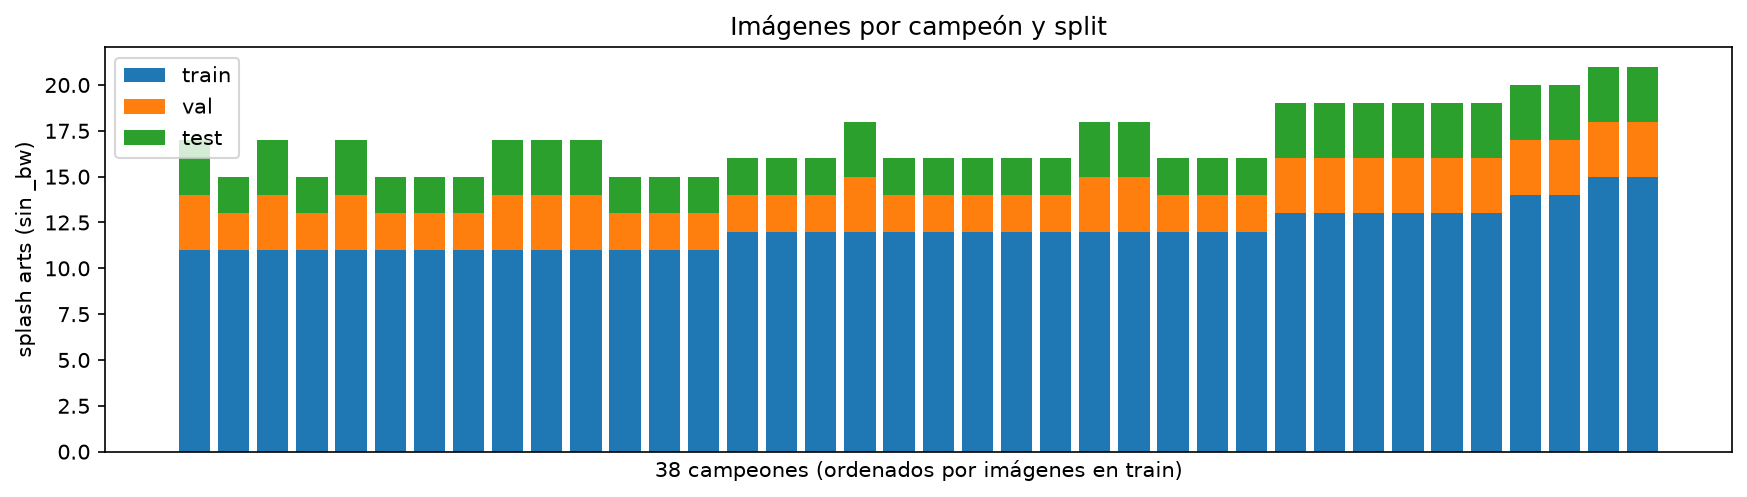
\includegraphics[width=\textwidth]{balance_splits.png}
  \caption{Imágenes por campeón en cada split. El desbalance entre clases es pequeño (11 a 15 en train).}
  \label{fig:balance}
\end{figure*}

Algo que hay que tener en cuenta en todo el reporte es que val y test tienen solo 95 imágenes cada uno, así que cada imagen vale alrededor de 0.011 de accuracy. Diferencias de una o dos imágenes entre versiones están dentro del ruido.

\subsection{Fan Arts y Cosplays}
\label{sec:fanarts}

Todas las versiones que fuimos probando (sección~\ref{sec:v5} en adelante) memorizan train y se quedan en alrededor de 0.3 en validación, y en la primera iteración el modelo mejoró en cuanto tuvo más imágenes por campeón. Por eso suponíamos que el límite era la falta de datos, y para comprobar si esa hipótesis era cierta decidimos agregar más imágenes de los mismos campeones.

Primero buscamos un dataset que ya tuviera fan arts de League of Legends, pero no encontramos ninguno. Lo único que había eran otros datasets de splash arts, con las mismas imágenes que ya teníamos, así que los descartamos. Al final juntamos las imágenes a mano en ArtStation, DeviantArt y Pinterest, buscando unas 10 por campeón en las que apareciera un solo campeón y que de preferencia fueran horizontales, como las splash. Hay fan arts de estilos muy distintos (realistas, chibi, anime) y también fotos de cosplay (Figura~\ref{fig:fanarts}).

De las 417 imágenes que juntamos quitamos 37. Con las mismas huellas que usamos para las splash grupales (MD5 y average hash) encontramos que 33 en realidad eran splash oficiales. De esas, 16 eran iguales a imágenes de validación o test, que hubieran inflado los resultados, y 17 a imágenes de train, que no aportaban nada nuevo. Las otras 4 eran imágenes repetidas. Quedaron 380 fan arts, entre 6 y 16 por campeón (10 en promedio).

Las fan arts solo se usan en train, así que validación y test siguen siendo las mismas splash y los resultados se pueden comparar con los de las versiones anteriores. Se procesan igual que las splash (384~px de alto con LANCZOS) y, como el modelo de ese momento entrenaba solo con imágenes en grises, se guardan solo en escala de grises.

\begin{figure*}[t]
  \centering
  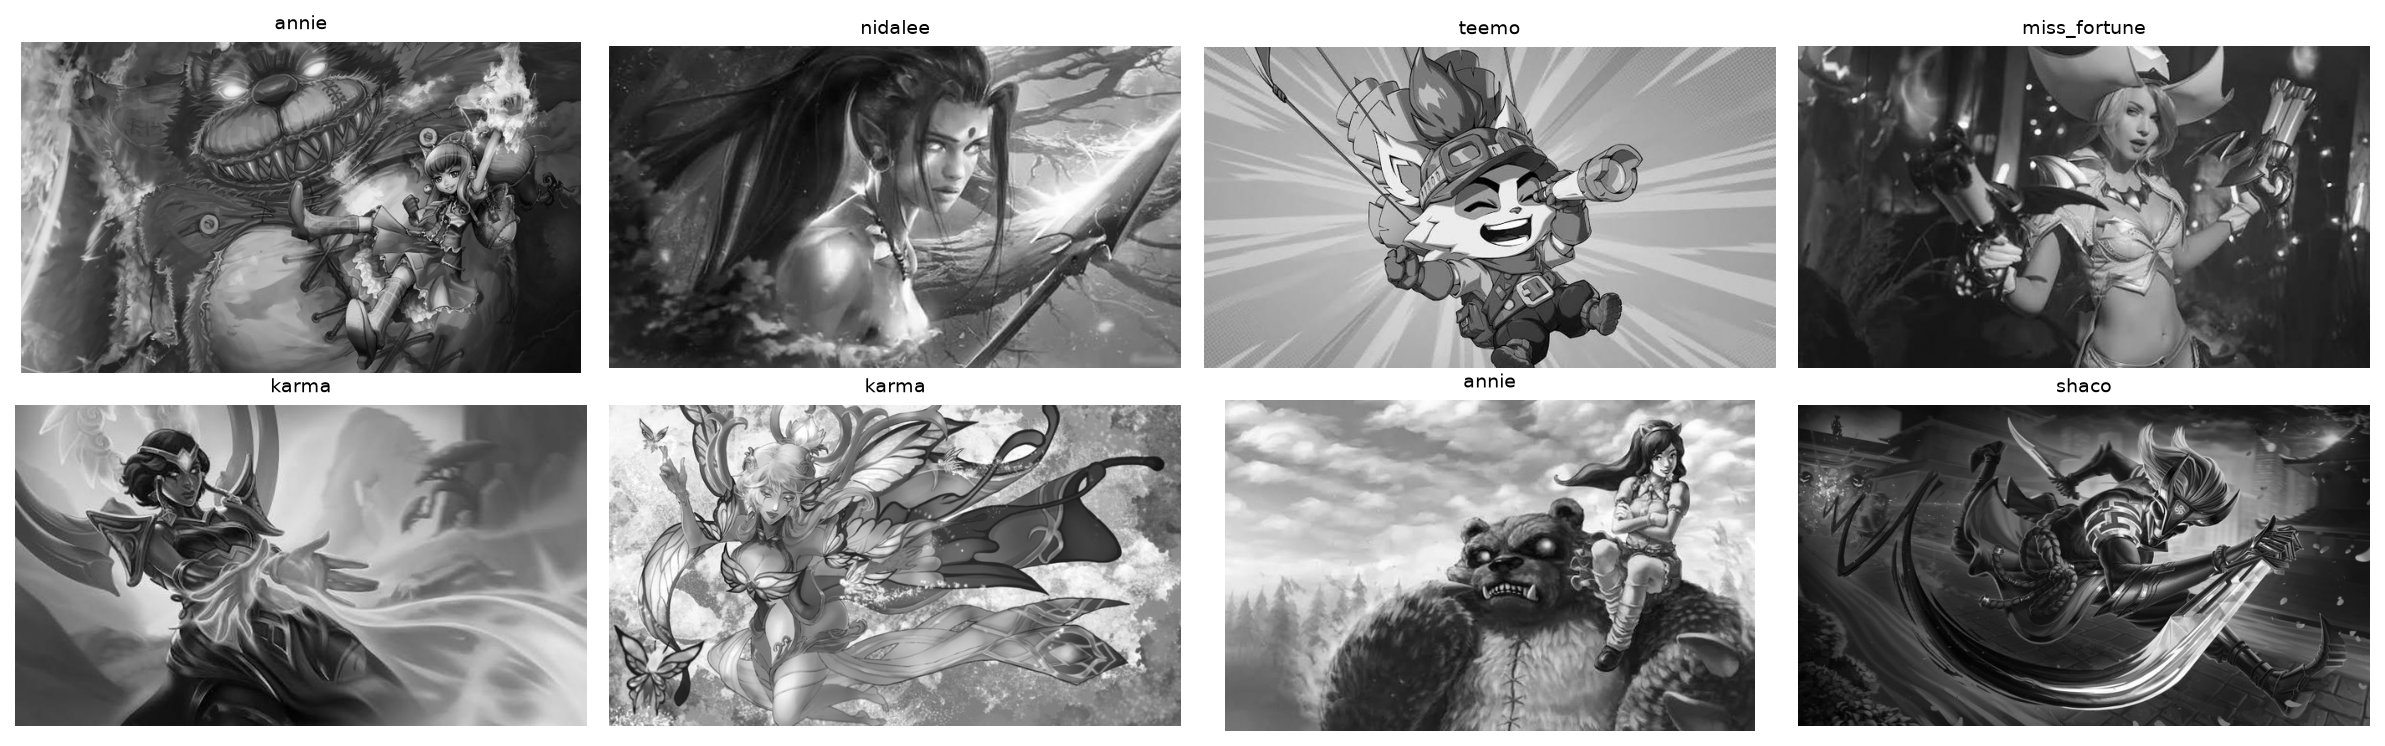
\includegraphics[width=\textwidth]{ejemplos_fan_arts.png}
  \caption{Ejemplos de fan arts y cosplays ya procesados en escala de grises.}
  \label{fig:fanarts}
\end{figure*}

\section{Transformación de Datos}

\subsection{De Imagen Ancha a Cuadrada}
\label{sec:cuadrado}

Las splash miden $1215\times717$ (una proporción de casi 1.7:1), pero las redes preentrenadas de Keras esperan entradas cuadradas, normalmente de $224\times224$. Comparamos tres formas de convertirlas (Figura~\ref{fig:cuadrado}):

\begin{itemize}
  \item \textbf{Estirar}: usa toda la imagen, pero deforma al campeón horizontalmente.
  \item \textbf{Recortar el centro}: no deforma, pero pierde cerca del 40\% del ancho, y en muchas splash el campeón no está centrado.
  \item \textbf{Letterbox} (rellenar con bordes negros): no deforma ni pierde nada, pero cerca del 40\% de la entrada son bordes y el campeón queda todavía más pequeño.
\end{itemize}

\begin{figure}[h]
  \centering
  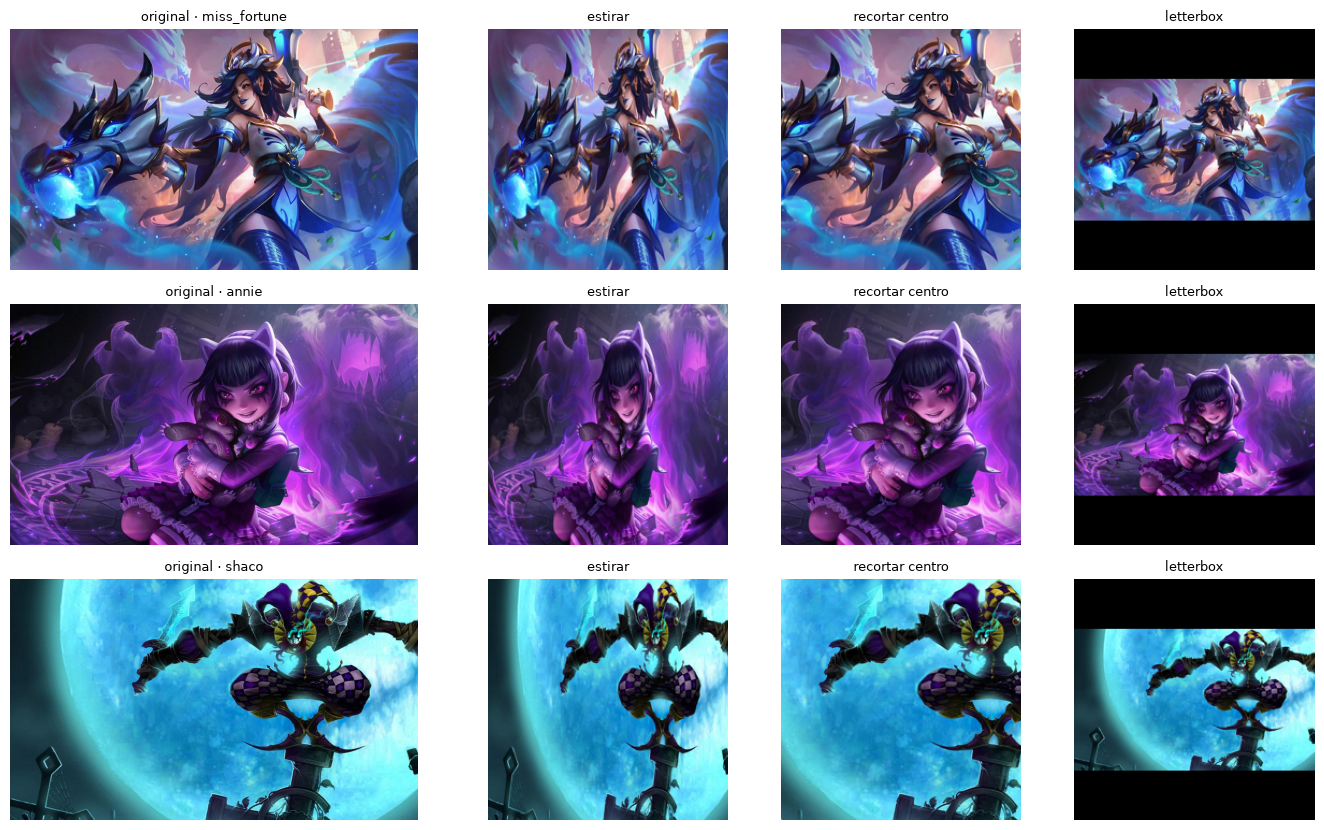
\includegraphics[width=\columnwidth]{formas_cuadrado.png}
  \caption{Tres formas de convertir una splash ancha en una entrada cuadrada.}
  \label{fig:cuadrado}
\end{figure}

En la segunda iteración probamos las tres con el mismo modelo. Estirar (F1 macro de validación 0.121) y recortar el centro (0.106) quedaron empatados dentro del ruido, y letterbox fue claramente peor (0.068). Nos quedamos con estirar para las versiones de 224~px. Lo que sí sacamos de esta prueba es que el tamaño con el que se ve al campeón parecía importar más que la forma de pasar a cuadrado, y eso es lo que nos llevó a la v5 (sección~\ref{sec:v5}).

\subsection{Reducción de Tamaño}

Guardar las splash a $1215\times717$ solo hacía más lenta la carga, así que las guardamos conservando la proporción con 384~px de alto (unos $651\times384$), que es la resolución más grande que usa cualquier versión. Usamos el filtro LANCZOS, que reduce sin generar artefactos. Las versiones de 224~px reducen la imagen al cargarla.

\subsection{Normalización}

La CNN desde cero recibe los pixeles normalizados a $[0,1]$ con una capa Rescaling(1/255). EfficientNet trae su propia normalización incluida en el modelo, así que a esas versiones les pasamos los pixeles en $[0,255]$ directamente.

\section{Construcción del Modelo}

\subsection{Métricas y Criterio de Selección}

Reportamos tres métricas para cada versión:

\begin{itemize}
  \item \textbf{Accuracy}: porcentaje de aciertos.
  \item \textbf{Top-5 accuracy}: si el campeón correcto está entre las 5 predicciones más probables. Con 38 clases es una medida útil de qué tan ``cerca'' está el modelo aunque falle.
  \item \textbf{F1 macro}: el promedio del F1 de cada campeón, todos con el mismo peso. Con esta métrica un modelo no puede verse bien acertando solo a unos cuantos campeones.
\end{itemize}

Todas las decisiones se tomaron con validación, usando la accuracy como criterio. Test se reporta para cada versión pero nunca se usó para elegir nada.

En la primera iteración usábamos EarlyStopping sobre val\_loss, y eso cortaba el entrenamiento demasiado pronto, porque la pérdida de validación sube en cuanto el modelo se vuelve demasiado confiado en sus errores, aunque el número de aciertos siga mejorando. En la v1 de esa iteración el modelo memorizó el 100\% de train en 3 épocas y se restauraron los pesos de la época 0. Por eso cambiamos a vigilar la accuracy de validación, que cuenta directamente los aciertos.

\subsection{Entrenamiento}

Todas las versiones se entrenan con la misma función, para que la comparación sea justa:

\begin{itemize}
  \item \textbf{Salida}: capa densa de 38 neuronas con softmax.
  \item \textbf{Pérdida}: sparse categorical crossentropy, porque las etiquetas son enteros:
  \begin{equation}
    J = -\frac{1}{m}\sum_{i=1}^{m}\log \hat{p}_{i,y_i}
  \end{equation}
  donde $\hat{p}_{i,y_i}$ es la probabilidad que el modelo le da al campeón correcto de la imagen $i$.
  \item \textbf{Optimizador}: Adam con learning rate de $10^{-3}$ (salvo el fine-tuning de la v4) y batches de 32.
  \item \textbf{EarlyStopping} sobre la accuracy de validación: para cuando deja de mejorar y restaura los pesos de la mejor época.
\end{itemize}

Cada versión se guarda en formato .keras (arquitectura y pesos) tal como se evaluó.

\subsection{v1: CNN desde Cero}

Como aproximación inicial armamos una CNN sencilla, con la misma estructura que el ejemplo de perros y gatos que vimos en clase: tres bloques de convolución $3\times3$ con ReLU (32, 64 y 128 filtros), cada uno seguido de un max pooling que reduce la resolución a la mitad, y al final un Flatten, una capa densa de 256 neuronas y la salida softmax. Tiene 22.3 millones de parámetros, casi todos en la capa densa (el Flatten genera 86,528 entradas).

La v1 llegó al 100\% de accuracy en train pero solo a 0.105 en validación (Figura~\ref{fig:v1}). Con 916 imágenes y 22 millones de parámetros, la red simplemente memorizó el conjunto de entrenamiento. El resultado está por encima del azar (0.026), pero muy lejos de ser útil.

\begin{figure*}[t]
  \centering
  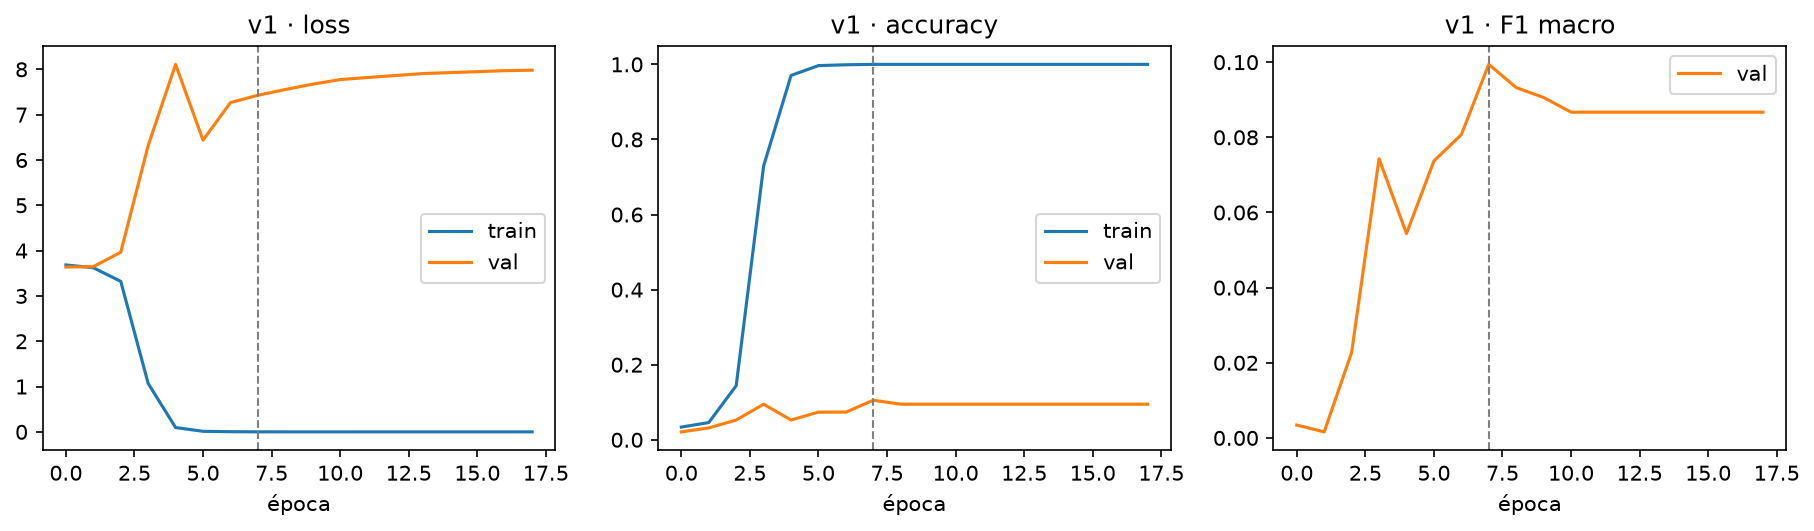
\includegraphics[width=\textwidth]{curvas_v1.png}
  \caption{Curvas de entrenamiento de la v1. Train llega al 100\% mientras la pérdida de validación se dispara, o sea que el modelo memoriza. La línea punteada marca la mejor época según la accuracy de validación.}
  \label{fig:v1}
\end{figure*}

\subsection{v2: Aumento de Datos y Dropout}

Para atacar el overfitting agregamos dos técnicas de regularización:

\begin{itemize}
  \item \textbf{Aumento de datos}: en cada época cada imagen llega con una transformación aleatoria distinta (volteo horizontal, rotación de hasta $\pm$18$^\circ$, zoom de $\pm$15\%, desplazamiento de $\pm$10\% y cambios de contraste), así el modelo no la puede memorizar (Figura~\ref{fig:aumento}). No usamos volteo vertical porque un campeón de cabeza no es una imagen realista. Estas capas solo actúan durante el entrenamiento.
  \item \textbf{Dropout} de 0.5 antes y después de la capa densa: apaga al azar la mitad de las neuronas en cada paso, para que el clasificador no dependa de unas pocas características.
\end{itemize}

\begin{figure*}[t]
  \centering
  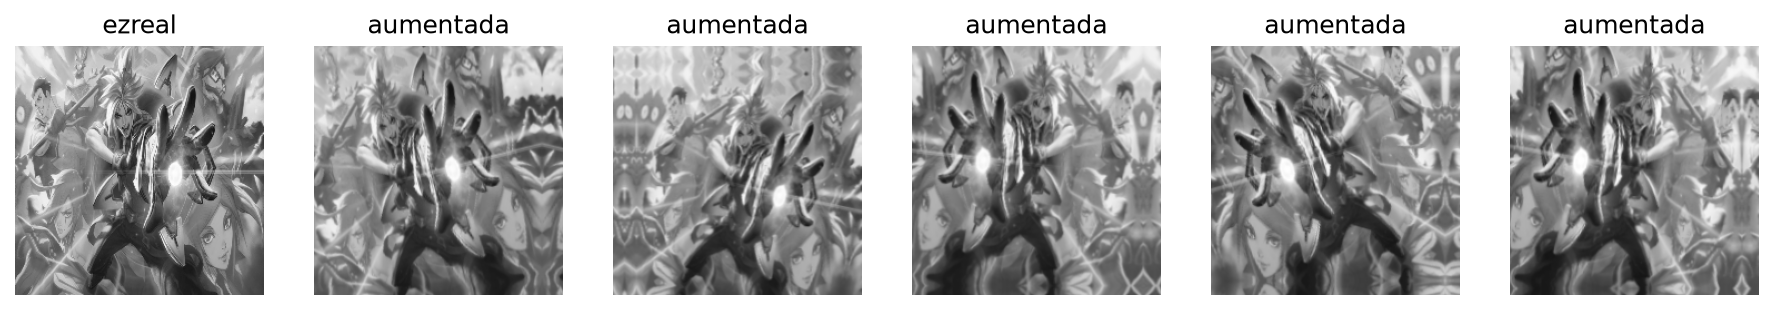
\includegraphics[width=\textwidth]{aumento_de_datos.png}
  \caption{Una imagen de train (en este caso una copia \_bw) y cinco versiones aumentadas al azar.}
  \label{fig:aumento}
\end{figure*}

El resultado fue peor, con 0.053 en validación y 0.037 en train (Figura~\ref{fig:v2}). Ya no memoriza, pero ahora tampoco aprende, porque con tan pocas imágenes la red desde cero no tiene de dónde sacar características generales (bordes, texturas, formas) y la regularización solo le quitó la capacidad de memorizar. Esto nos dejó claro que el problema no se resolvía regularizando una red desde cero, sino dándole al modelo características que ya sepan ``ver''.

\begin{figure*}[t]
  \centering
  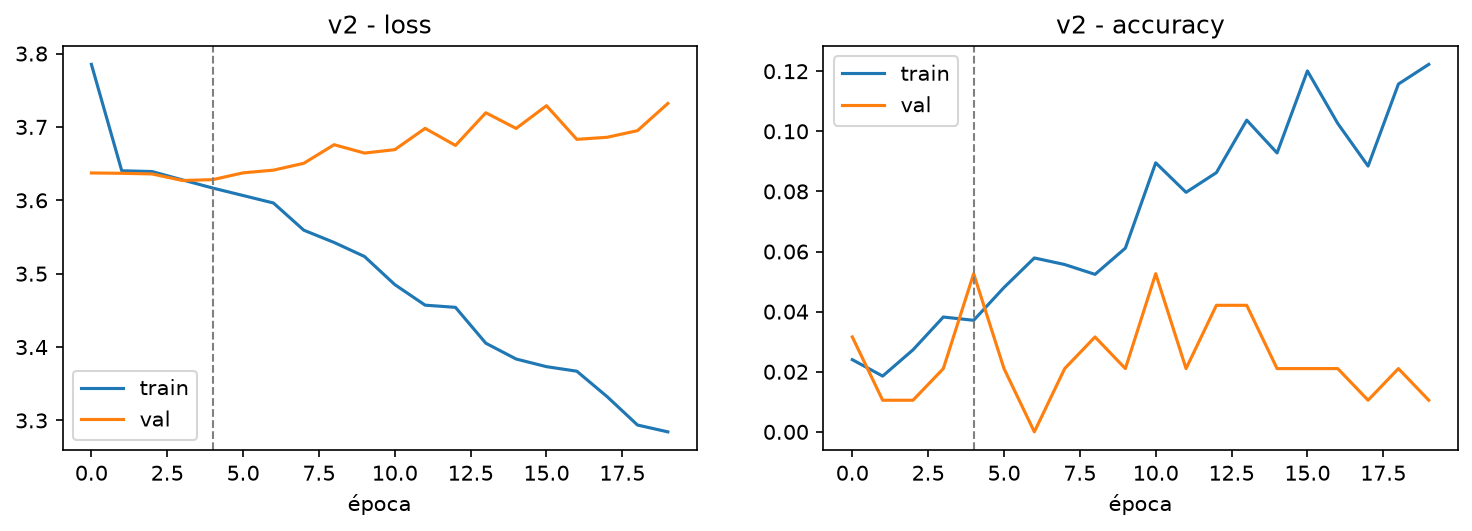
\includegraphics[width=\textwidth]{curvas_v2.png}
  \caption{Curvas de entrenamiento de la v2. Con aumento de datos y Dropout, la accuracy de train no pasa de 0.12, así que el modelo deja de memorizar pero tampoco aprende.}
  \label{fig:v2}
\end{figure*}

\subsection{v3: Transfer Learning con EfficientNetB0}

El transfer learning reutiliza una red ya entrenada con ImageNet (1.4 millones de imágenes), que ya sabe extraer bordes, texturas y formas, y solo entrena un clasificador nuevo encima. Elegimos EfficientNetB0~\cite{efficientnet} porque en el diagnóstico de la Tabla~\ref{tab:backbones} fue la de mejores características congeladas, y porque es una red ligera que corre bien en CPU. EfficientNet escala de forma balanceada la profundidad, el ancho y la resolución, y usa bloques MBConv con convoluciones depthwise y atención por canal.

\begin{itemize}
  \item include\_top=False quita el clasificador original de 1000 clases de ImageNet.
  \item base.trainable = False congela los 4 millones de parámetros de la base. Solo se entrenan 48,678.
  \item GlobalAveragePooling2D resume cada mapa de características en un número, en lugar del Flatten de la v1, que generaba 22 millones de parámetros.
  \item Mantenemos el aumento de datos y un Dropout de 0.3 antes de la salida.
\end{itemize}

La v3 subió a 0.189 en validación (F1 0.165) y a 0.347 en top-5, con mucho menos overfitting que la v1 (0.586 en train).

\subsection{v4: Fine-Tuning}

Con el clasificador de la v3 ya entrenado, descongelamos el último bloque de EfficientNetB0 para que también se ajustara a las splash arts. Las primeras capas detectan cosas genéricas que sirven para cualquier imagen, mientras que las últimas detectan patrones más específicos de ImageNet, que son las que conviene adaptar.

\begin{itemize}
  \item Descongelamos desde block6a (bloques 6 y 7 y la convolución final), que son 59 de 238 capas y 3.2 millones de parámetros. Descongelar más significaba más parámetros que reentrenar con pocos datos y más riesgo de perder lo aprendido en ImageNet.
  \item Usamos un learning rate más bajo ($10^{-5}$) para que los pesos de la base cambiaran poco.
  \item Dejamos congeladas las capas de Batch Normalization, para que solo se ajustaran las convoluciones.
  \item No empezamos de cero, seguimos entrenando el mismo modelo de la v3.
\end{itemize}

La v4 mejoró un poco en validación (0.200, F1 0.168), pero test no se movió (0.137 en ambas). En la segunda iteración ya habíamos visto lo mismo, cambiar de backbone, la forma de pasar a cuadrado o el aumento de datos no movía test de alrededor de 0.17, así que el límite tenía que estar en otra parte.

\subsection{v5: Multi-Recorte a 384 px}
\label{sec:v5}

En la prueba de las formas de pasar a cuadrado (sección~\ref{sec:cuadrado}), letterbox, que deja al campeón más pequeño, fue la peor. Eso nos hizo pensar que el tamaño con el que el modelo ve al campeón importa, y al aplastar una splash de 1.7:1 a $224\times224$ el campeón queda pequeño y deformado.

La idea de la v5 fue no aplastar la imagen. Dividimos la splash de $651\times384$ en tres recortes cuadrados de $384\times384$ (izquierda, centro y derecha, que se traslapan), pasamos cada uno por la misma EfficientNetB0 y concatenamos los tres vectores de características (Figura~\ref{fig:multirecorte}). Así el campeón se ve sin deformar y con casi 1.7 veces más resolución, y el clasificador sabe en qué zona de la imagen apareció cada característica. En un diagnóstico previo, concatenar dio mejor F1 en validación (0.274) que promediar los tres recortes (0.226).

En Keras armamos los recortes dentro del propio modelo:

\begin{itemize}
  \item Tres capas Cropping2D toman la misma entrada de $651\times384$ y le quitan columnas a la derecha (recorte izquierdo), a ambos lados (centro) o a la izquierda (recorte derecho), dejando cuadrados de $384\times384$.
  \item Los tres recortes pasan por la misma instancia de EfficientNetB0, así que comparten pesos, o sea que el modelo no tiene más parámetros que con una sola entrada, solo procesa la imagen tres veces.
  \item Una capa Concatenate junta las tres salidas siempre en el mismo orden (izquierda, centro, derecha). Por eso el clasificador sabe de qué zona viene cada característica.
\end{itemize}

\begin{figure*}[t]
  \centering
  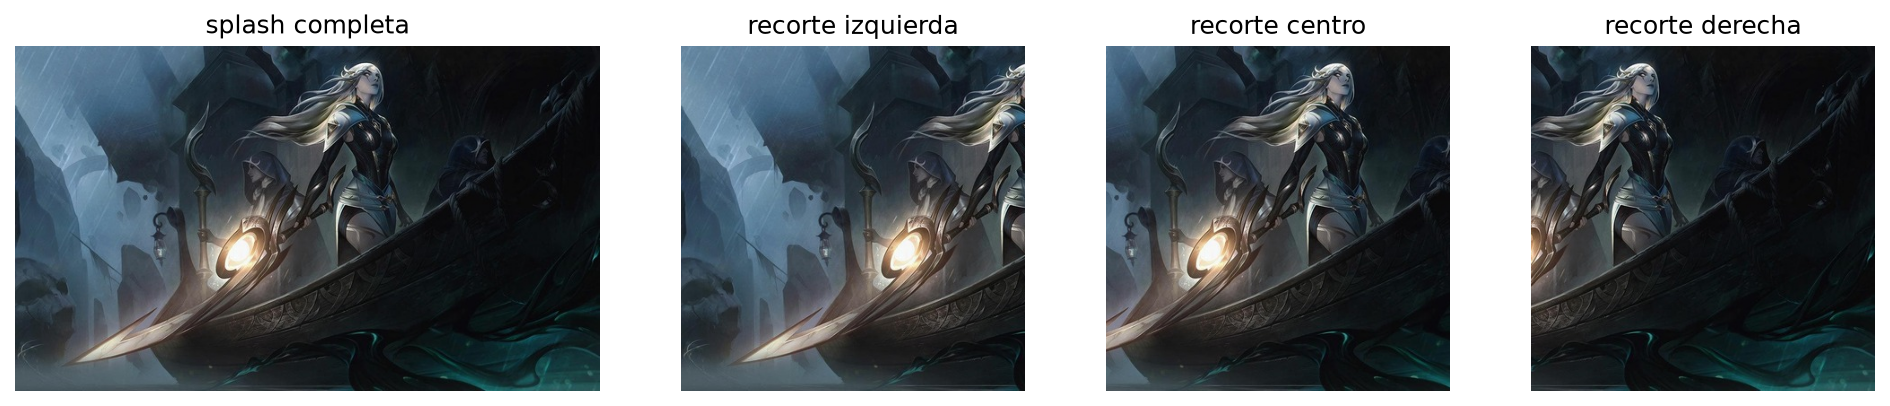
\includegraphics[width=\textwidth]{multirecorte.png}
  \caption{Una splash completa y sus tres recortes cuadrados de $384\times384$.}
  \label{fig:multirecorte}
\end{figure*}

Procesar tres recortes de 384~px por imagen en cada época era muy lento en CPU, así que usamos la base como extractor de características fijo, que es una de las formas de transfer learning que vimos en clase. Como está congelada, sus características no cambian entre épocas, así que las calculamos una sola vez ($3\times1280 = 3840$ por imagen) y después entrenamos solo el clasificador (Dropout de 0.3 y la capa softmax), en segundos por época.

El costo es que no se puede usar aumento de datos aleatorio. En su lugar agregamos una copia volteada horizontalmente de cada imagen de train (1,832 ejemplos). En la segunda iteración habíamos visto que quitar el aumento aleatorio no empeoraba los resultados, así que no perdíamos mucho.

Al final unimos el extractor y el clasificador en un solo modelo que recibe la splash completa. La v5 fue el salto más grande, con 0.242 en validación y en test, y el top-5 de validación pasó de 0.368 a 0.589. Aun así, la v5 llega al 99\% en train, así que cambiar la entrada ayudó pero el overfitting seguía ahí.

\section{¿El Modelo Depende del Color?}

Entre las skins de un campeón lo que más cambia es la paleta de colores, mientras que la forma, la silueta y las proporciones se mantienen. Si el clasificador se apoya en el color, estaría aprendiendo pistas que no se repiten de una skin a otra.

\subsection{Diagnóstico}

Para probarlo evaluamos la v5, tal como se entrenó (color más copias \_bw), con validación y test convertidos a escala de grises. Si el modelo dependiera del color, los resultados deberían bajar.

\begin{table}[h]
  \centering
  \begin{tabular}{lcc}
    \toprule
    \textbf{Split} & \textbf{Color} & \textbf{Grises} \\
    \midrule
    Validación & 0.242 (23) & \textbf{0.295 (28)} \\
    Test       & 0.242 (23) & \textbf{0.295 (28)} \\
    \bottomrule
  \end{tabular}
  \caption{Accuracy (y aciertos de 95) de la v5 evaluada a color y en escala de grises.}
  \label{tab:grises}
\end{table}

Los resultados no bajaron, al contrario, en los dos splits el modelo acierta 5 imágenes más en grises que a color (Tabla~\ref{tab:grises}). O sea que el modelo no depende del color, y más bien el color de las skins le estorba, así que decidimos entrenar directamente en grises.

\subsection{v6: Entrenar y Predecir en Escala de Grises}

Si el clasificador solo ve imágenes en grises al entrenar, no puede aprender pistas de color y se tiene que apoyar en la forma del campeón. La v6 es la misma v5, cambiando solo los datos: en train usa solo las copias \_bw y su volteo, y validación y test se convierten a grises antes de predecir.

La v6 fue la mejor versión en validación hasta ese punto, con accuracy de 0.316 (30 aciertos contra 23 de la v5) y F1 macro de 0.278 (contra 0.207). En test también mejoró a la v5 (0.263 contra 0.242). Lo único que no mejoró fue el top-5 de validación (0.579 contra 0.589), o sea que cuando el modelo en grises falla, el campeón correcto queda un poco menos veces entre las 5 primeras opciones.

\subsection{v7: Color y Grises con más Peso a los Grises}

Quitar el color por completo también quita las pistas de color que sí se mantienen entre skins, como el tono de piel de algunos campeones. Para buscar un punto intermedio, la v7 entrena con todas las imágenes de train (a color y \_bw, más sus volteos), pero cada imagen a color cuenta la mitad en la pérdida, y se evalúa en grises igual que la v6.

Para eso usamos sample\_weight de Keras~\cite{keras}, que le asigna un peso a cada ejemplo dentro de la pérdida. Las copias \_bw tienen peso 1 y las imágenes a color (con sus volteos) peso 0.5. De esta forma, equivocarse en una imagen a color mueve los pesos la mitad que equivocarse en una en grises, así que el modelo sigue viendo el color, pero lo que más le conviene aprender son las características que también funcionan en grises. Con peso 1 para todas, el entrenamiento sería el de la v5, y con peso 0 para las de color, prácticamente el de la v6, así que la v7 queda entre las dos. En Keras basta con que el dataset regrese (x, y, w) en lugar de (x, y).

Fijamos el peso en 0.5 antes de ver resultados, porque probar varios pesos y quedarnos con el mejor hubiera sido ajustar a validación con solo 95 imágenes.

La v7 quedó prácticamente empatada con la v6: 29 aciertos contra 30 en validación, con un F1 un poco mayor (0.283 contra 0.278) y mejor top-5 (0.600 contra 0.579), lo que sugiere que el color sí aporta como pista secundaria. Pero las diferencias son de una imagen, dentro del ruido, y con nuestra regla (elegir por accuracy en validación) gana la v6, que además es más simple porque no necesita las imágenes a color ni un peso que ajustar. En test la v7 salió mejor (0.295 contra 0.263), pero test no se usa para elegir, ya que hacerlo convertiría a test en una segunda validación y su resultado dejaría de ser una medida confiable.

\subsection{v8: Fan Arts en Train (Modelo Final)}

Con la v6 como base probamos la hipótesis de la falta de datos. La v8 es exactamente la misma v6 (mismo extractor, mismo clasificador y mismo entrenamiento), y lo único que cambia es que a train le agregamos las 380 fan arts y cosplays de la sección~\ref{sec:fanarts} con sus volteos, lo que da 1,676 ejemplos contra 916 de la v6.

La v8 fue la mejor versión en validación, con accuracy de 0.389 (37 aciertos contra 30 de la v6), F1 macro de 0.374 (contra 0.278) y top-5 de 0.653 (contra 0.579). Esta mejora la conseguimos sin cambiar nada del modelo, solo dándole más imágenes, así que la hipótesis de que el límite eran los datos era cierta.

En test casi no hubo cambio. La accuracy quedó igual (25 aciertos de 95), aunque no son las mismas imágenes, ya que la v8 acierta 6 que la v6 fallaba y falla otras 6 que la v6 acertaba. El F1 macro subió un poco (0.242 contra 0.230) y el top-5 bajó una imagen (0.516 contra 0.526). Parte de la diferencia con validación viene de que elegimos la mejor época con validación, y su accuracy brinca entre 0.33 y 0.39 de una época a otra, mientras que test no se usó para elegir nada. Aun así, con nuestra regla de selección la v8 es la mejor versión, así que es nuestro modelo final.

\subsection{v9: Modelo para la Interfaz Web}

En clase vimos que, una vez que el modelo ya no tiene overfitting, se puede reentrenar con todo el dataset. Nuestro caso no cumple del todo esa condición, porque la v8 llega al 99\% en train, pero como acabamos de ver con las fan arts, el overfitting viene sobre todo de que hay muy pocas imágenes por campeón, así que darle más imágenes es justo lo que más le puede ayudar. La v9 es exactamente la configuración de la v8 (mismo extractor, mismo clasificador, mismo learning rate y las 23 épocas de su mejor resultado), entrenada en grises con train, fan arts, validación y test y sus volteos, lo que da 2,056 ejemplos contra 1,676 de la v8, unas 5 splash más por campeón.

La v9 es la que usa la interfaz web, porque con más imágenes debería generalizar mejor. Pero no es el modelo final del reporte, porque como ya no queda ninguna imagen que no haya visto, no hay forma de medirla y sus resultados no se pueden comparar con los de las demás versiones. Las métricas que reportamos son las de la v8, que es el modelo que entrenamos solo con train y fan arts, elegimos con validación y medimos en test.

\section{Visualización y Resultados}

La Tabla~\ref{tab:resultados} resume todas las versiones y la Figura~\ref{fig:comparacion} compara las que tienen métricas de validación.

\begin{table*}[t]
  \centering
  \small
  \resizebox{\textwidth}{!}{%
  \begin{tabular}{llcccccc}
    \toprule
    \textbf{Versión} & \textbf{Cambio} & \textbf{Train acc} & \textbf{Val acc} & \textbf{Val F1} & \textbf{Test acc} & \textbf{Test top-5} & \textbf{Test F1} \\
    \midrule
    v1 & CNN desde cero ($224\times224$)                      & 1.000 & 0.105 & 0.099 & 0.105 & 0.305 & 0.105 \\
    v2 & v1 + aumento de datos + Dropout                      & 0.037 & 0.053 & 0.020 & 0.032 & 0.179 & 0.006 \\
    v3 & EfficientNetB0 congelada + aumento                   & 0.586 & 0.189 & 0.165 & 0.137 & 0.400 & 0.109 \\
    v4 & v3 + fine-tuning desde block6a              & 0.604 & 0.200 & 0.168 & 0.137 & 0.389 & 0.096 \\
    v5 & 3 recortes de 384 px, EfficientNetB0 como extractor  & 0.991 & 0.242 & 0.207 & 0.242 & 0.505 & 0.227 \\
    v6 & v5 entrenada y evaluada en grises                   & 0.991 & 0.316 & 0.278 & 0.263 & \textbf{0.526} & 0.230 \\
    v7 & v5 color (peso 0.5) + grises, evaluada en grises     & 0.991 & 0.305 & 0.283 & \textbf{0.295} & 0.505 & \textbf{0.279} \\
    \textbf{v8} & \textbf{v6 + fan arts en train (final)}    & 0.995 & \textbf{0.389} & \textbf{0.374} & 0.263 & 0.516 & 0.242 \\
    v9 & v8 reentrenada con train + val + test (web)          & 0.992 & --    & --    & --    & --    & -- \\
    \bottomrule
  \end{tabular}}
  \caption{Resultados de todas las versiones. El azar con 38 clases es 0.026. La v9 se entrenó con todas las imágenes, así que no tiene métricas de validación ni de test.}
  \label{tab:resultados}
\end{table*}

\begin{figure}[h]
  \centering
  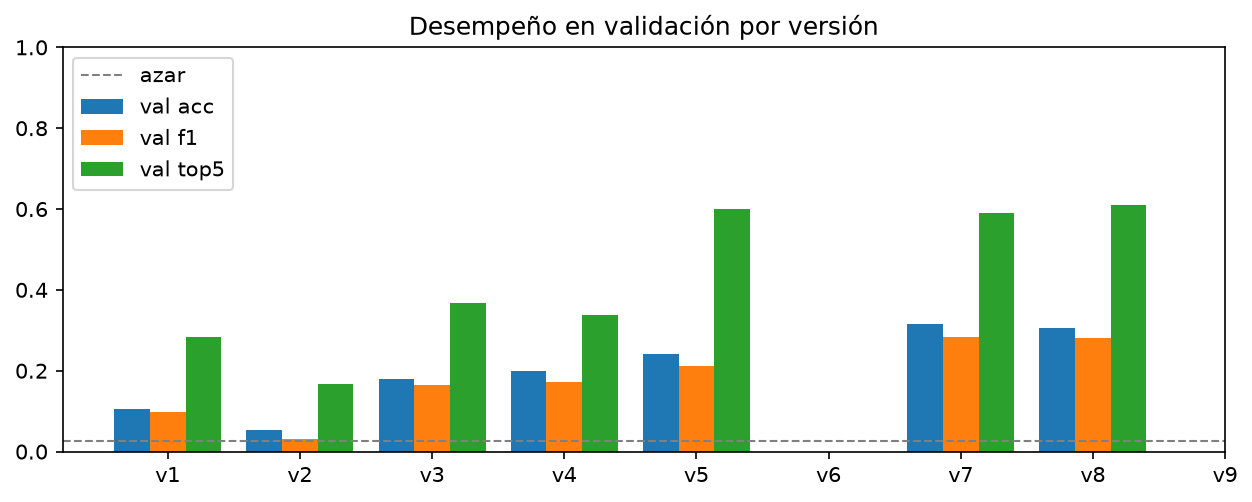
\includegraphics[width=\columnwidth]{comparacion_versiones.png}
  \caption{Accuracy, F1 macro y top-5 en validación por versión. La línea punteada es el azar.}
  \label{fig:comparacion}
\end{figure}

Viendo la tabla completa, hay tres cosas que destacan:

\begin{itemize}
  \item \textbf{El tamaño con el que se ve al campeón importó más que la arquitectura.} Entre v3 y v4 (y en las iteraciones anteriores, cambiando de backbone) validación se movió poco y test nada, mientras que dividir la splash en tres recortes a mayor resolución (v5) fue el salto más grande.
  \item \textbf{El color de las skins confunde al modelo.} Evaluar en grises mejora a un modelo entrenado a color, y entrenar solo en grises subió validación de 0.242 a 0.316.
  \item \textbf{El límite son los datos.} Todas las versiones con transfer learning a 384~px llegan a cerca del 99\% en train. En la primera iteración, pasar de unas 9 a unas 12 imágenes por campeón (de 107 a 38 campeones) subió validación de 0.116 a 0.263 con el mismo modelo, y al agregar las fan arts (v8) subió de 0.316 a 0.389, también sin cambiar el modelo, aunque en test la accuracy no se movió.
\end{itemize}

\subsection{Análisis del Modelo Final en Test}

El modelo final (v8) acierta 25 de las 95 imágenes de test, y en el 51.6\% de los casos el campeón correcto está en su top 5. El desempeño por campeón es muy desigual, Leona llega a un F1 de 0.80 y Shaco, Warwick, Blitzcrank, Soraka y Sona a 0.67, mientras que 19 de los 38 campeones tienen F1 de 0 (entre ellos Ahri, Veigar, Sivir, Riven, Master Yi, Katarina, Karma y Janna). Hay que tomar esto con cuidado, porque cada campeón tiene solo 2 o 3 imágenes en test.

La matriz de confusión (Figura~\ref{fig:confusion}) muestra que los errores no se reparten al azar, ya que el modelo tiene campeones ``comodín'' a los que manda muchas imágenes que no reconoce, como Irelia (7 errores), Miss Fortune, Sivir y Vayne (5 cada uno) y Master Yi (4). Son campeones humanoides, una silueta que se parece a la de muchos otros. Master Yi es un caso claro, recibe 4 predicciones equivocadas y no acierta ninguna de sus propias imágenes.

\begin{figure}[h]
  \centering
  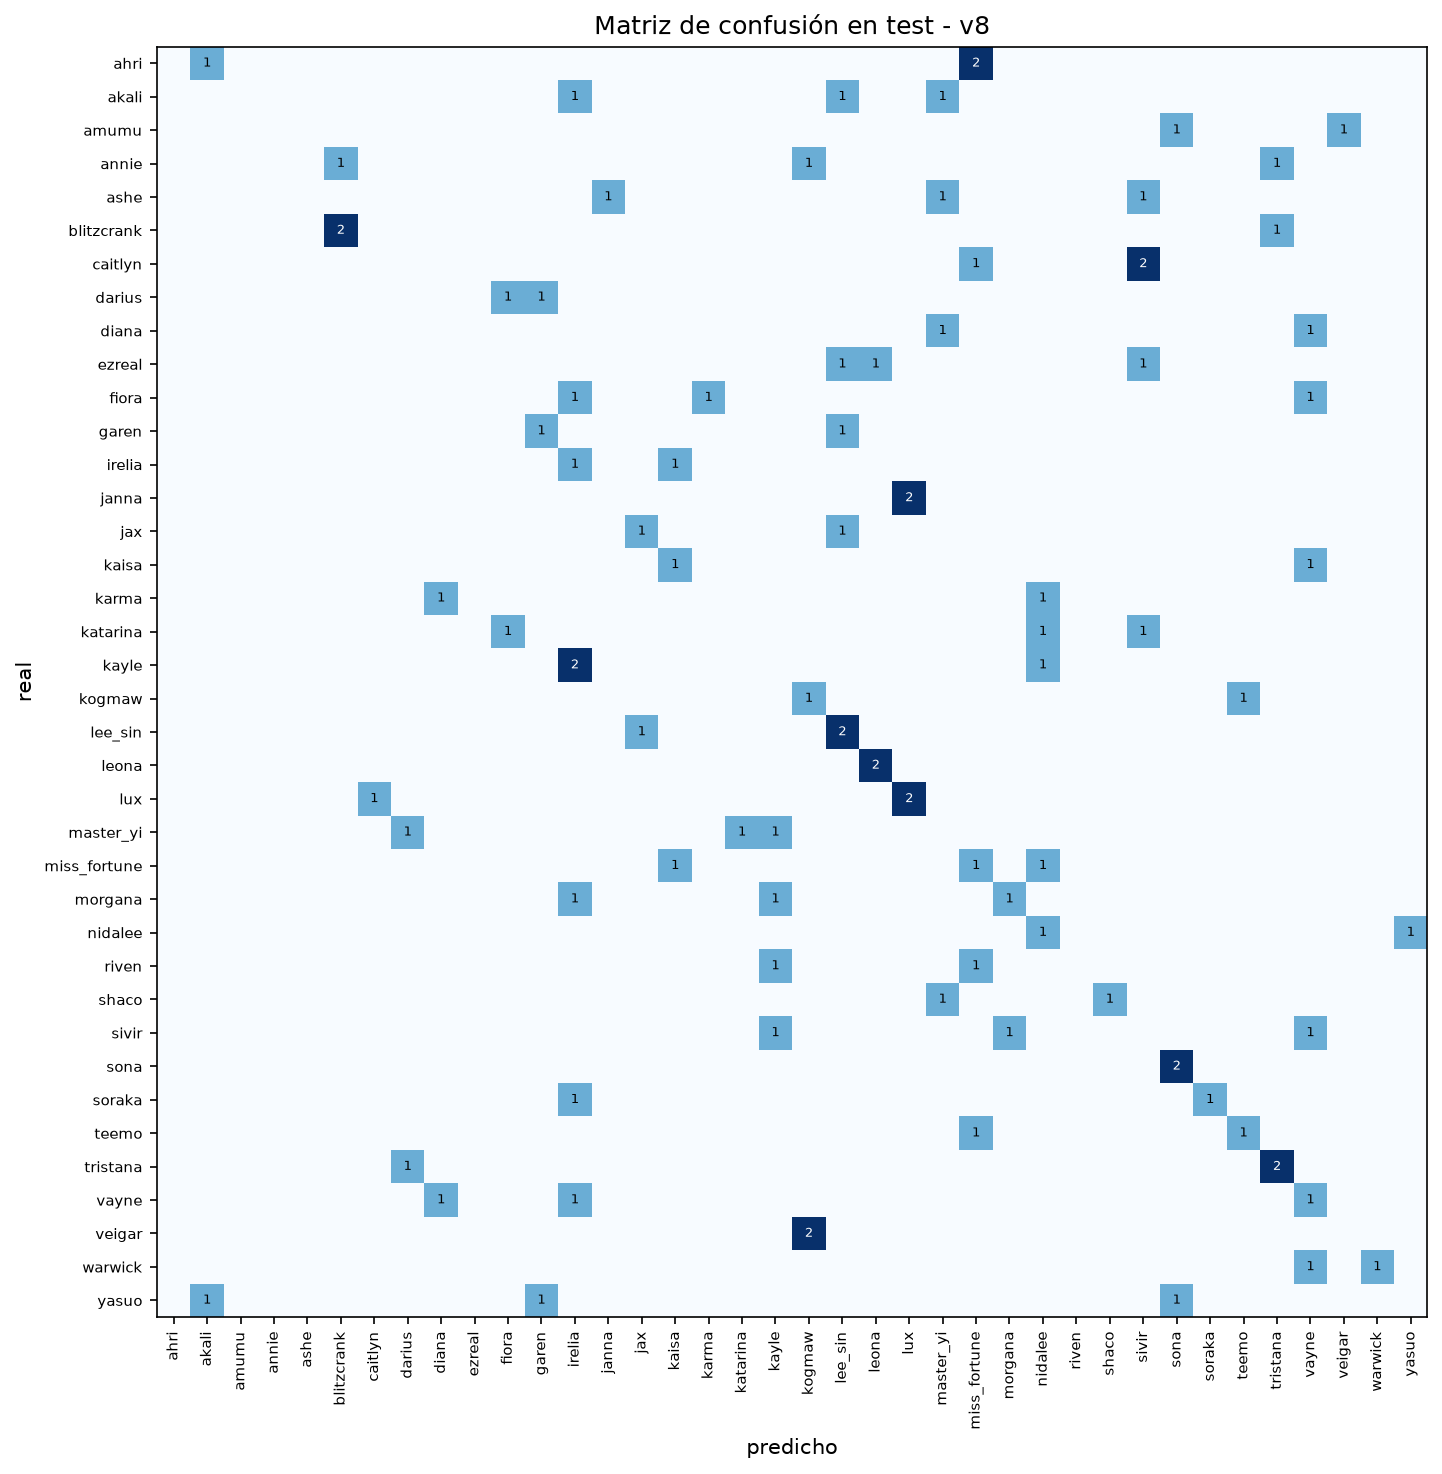
\includegraphics[width=0.85\columnwidth]{matriz_confusion.png}
  \caption{Matriz de confusión del modelo final en test.}
  \label{fig:confusion}
\end{figure}

La Figura~\ref{fig:ejemplos} muestra predicciones sobre imágenes de test. El modelo acierta con más seguridad a campeones de silueta única, como Kog'Maw (87\%), y falla con humanoides parecidos entre sí, por ejemplo confunde a Morgana con Irelia, a Vayne con Diana y a Caitlyn con Sivir. Algunos errores son con bastante seguridad, como Yasuo confundido con Sona (76\%) o Veigar con Kog'Maw (55\%), dos campeones pequeños. También se ve un caso de splash con varios personajes (Annie con un personaje grande al lado), donde el modelo responde por otro campeón.

\begin{figure*}[t]
  \centering
  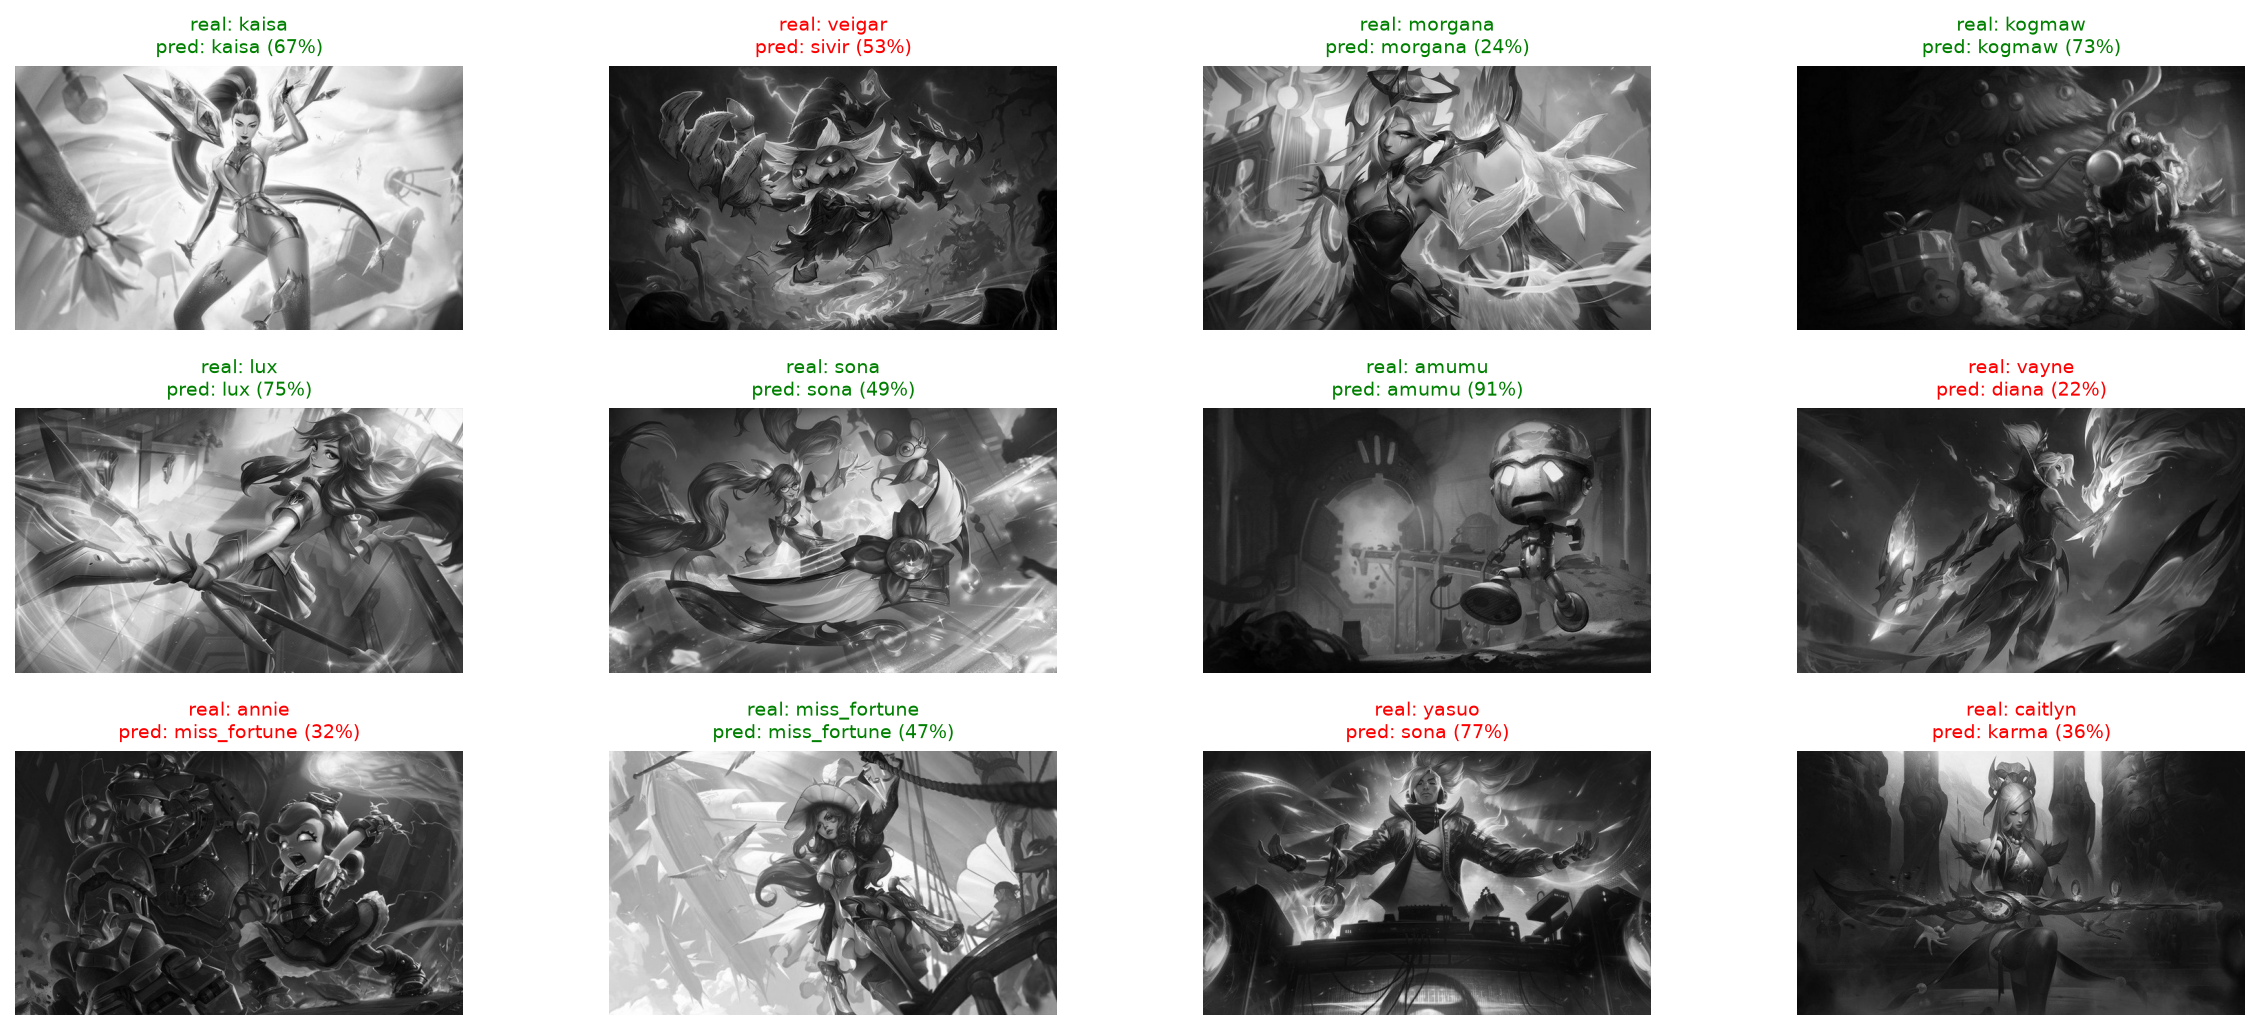
\includegraphics[width=0.85\textwidth]{ejemplos_test.png}
  \caption{Predicciones del modelo final (v8) sobre imágenes de test, ya convertidas a escala de grises. En verde los aciertos y en rojo los errores, con la probabilidad que el modelo le dio a su predicción.}
  \label{fig:ejemplos}
\end{figure*}

\section{Interfaz Web}

Para mostrar cómo funciona el modelo armamos una interfaz web sencilla, que usa la v9 (la configuración del modelo final reentrenada con todas las imágenes, incluidas las fan arts). El modelo se guarda en formato .keras junto con un archivo metadata.json que tiene la lista de campeones, el tamaño de entrada y si el modelo espera la imagen en escala de grises. Un servidor en Python (src/app.py) carga el modelo una sola vez, recibe las imágenes que sube el usuario, les aplica el mismo preprocesamiento del entrenamiento y regresa el top 5 de campeones con su probabilidad.

Como el modelo se entrenó con splash horizontales, las imágenes con una proporción muy distinta (verticales o cuadradas) no se pueden estirar a $651\times384$ sin deformarlas mucho. Si la proporción se aleja más de 15\% de la de una splash, la imagen se coloca completa con bordes negros. Las imágenes que usamos para probar la interfaz son externas al dataset y no son parte de la evaluación del modelo, que es la de la v8 en test.

\section{Conclusiones}

Construimos un clasificador que reconoce a 38 campeones de League of Legends a partir de sus splash arts con 0.263 de accuracy, 0.516 de top-5 y 0.242 de F1 macro en test, 10 veces más que el azar. Es un resultado moderado, pero tiene sentido si se considera que hay solo 12 skins y 10 fan arts por campeón en train, y que no comparten colores, ropa ni fondo.

Las mejoras más grandes salieron de revisar por qué fallaba el modelo y no de cambiar de arquitectura. Así fue como decidimos limpiar las splash grupales que eran imposibles de aprender, reducir los campeones cuando vimos que todas las redes llegaban al mismo techo, mostrarle al campeón a mayor resolución cuando vimos que el tamaño con el que lo ve importaba, quitar el color cuando vimos que le estorbaba y agregar fan arts y cosplays cuando vimos que todas las versiones memorizaban train.

Nuestra hipótesis era que el límite del modelo estaba en la falta de datos, y con las fan arts pudimos ver que era cierta, ya que con más imágenes por campeón el mismo modelo subió en validación de 0.316 a 0.389 y el F1 macro de 0.278 a 0.374. En test la accuracy quedó igual y el F1 subió un poco, pero con solo 95 imágenes una diferencia de pocas imágenes está dentro del ruido. Lo que más podría seguir ayudando es conseguir todavía más imágenes por campeón, lo que además permitiría volver a incluir a los campeones que quitamos.

\begin{thebibliography}{9}
\small

\bibitem{dataset}
Elimam, H. E. (n.d.). \textit{League of Legends Champions Visual Data}. Kaggle. \url{https://www.kaggle.com/datasets/houssemeddineelimam/league-of-legends-champions-visual-data}

\bibitem{efficientnet}
Tan, M., \& Le, Q. V. (2019). EfficientNet: Rethinking model scaling for convolutional neural networks. Proceedings of the 36th International Conference on Machine Learning, 6105--6114.

\bibitem{keras}
Keras. (n.d.). Model training APIs. \url{https://keras.io/api/models/model_training_apis/}

\end{thebibliography}

\end{document}
